\subsection{Private chain}
\label{sec:priv-chain}

Every educator has a private chain. It stores the data about students, and can
generate answers for the queries described above.

Private chain comprises of two main data structures:
\begin{itemize}
\item Set of transactions batched into blocks. Every block contains a list of
  transactions packed into a Merkle tree.
\item Links to the transactions stored in the B+-tree with keys (studentId,
  studentGrade). Indexes constructed in such a way that more popular activities
  go first.
\end{itemize}

The structure of the private block is shown in Figure~\ref{fig:privateblocks}.
The block consists of a public \textit{header} that the Educators relay to the
Witnesses, and the private \textit{body} that remains in the educational
institute until it receives a data disclosure request.

\begin{figure}[ht]
\centering
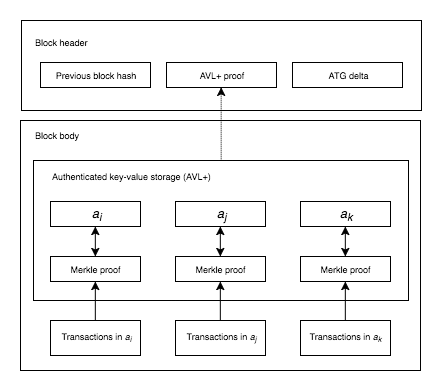
\includegraphics[width=0.8\textwidth]{private-blocks}
\caption{Private block structure}
\label{fig:privateblocks}
\end{figure}

During the educational process the Educators emit atomic \textit{private
  transactions}. These transactions represent the modifications to the journal of
academic achievements (thus, making a transaction means appending the data to
the journal). The transactions can be of the following types:

\begin{itemize}
\item student enrolls in a course;
\item student gets an assignment;
\item student submits an assignment;
\item student gets a grade for an assignment;
\item student gets a final grade for the course.
\end{itemize}

The first two types should be intiated by a student, and should include
student's signature to prevent spam from partially-honest educator. The
structure of the transaction is shown in Figure~\ref{fig:private-transactions}.

Let us denote an $i$-th transaction in a block as $T_{priv}^i$. The Educators
group the transactions that occured during the current block time slot, and
construct a Merkle tree \cite{merkle1989certified} for these journal
modifications:

\begin{equation}
M_{priv} = \MerkleTree(\{\ T_{priv}^i\ \})
\end{equation}

\begin{figure}[ht]
\centering
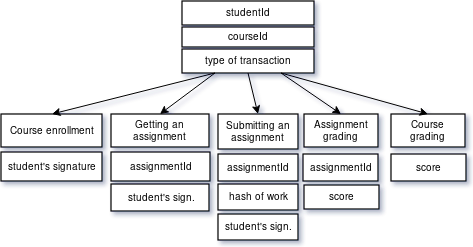
\includegraphics[width=0.8\textwidth]{private-transactions}
\caption{Transaction structure}
\label{fig:private-transactions}
\end{figure}

The Educator's private block body comprises an ordered set of
Merkle-authenticated transactions. These transactions are indexed so that the
Educator can quickly find a particular transaction that satisfies some
predicate.

The private block header consists of the transactions Merkle root along with the
previous block hash and the information on the Activity Type Graph modifications
(ATG delta). The \textit{ATG delta} part allows the Educators to inform the
Witnesses of the modifications to the courses they teach. The ATG delta is a
pair of sets $\Delta_A = (\Delta_{A+}, \Delta_{A-})$, where $\Delta_{A+}$ is a
set of subjects for which Educator starts a course and $\Delta_{A-}$ is a set of
subjects for which Educator closes a course.

An Educator collects private transactions into the blocks with no more than $K_{max}$
transactions per each block. After that, an Educator submits signed block header
to the Witnesses so that private transactions can be confirmed by the public
chain. Thus, the private blocks form a publicly verifiable chain of events.

\begin{figure}[ht]
\centering
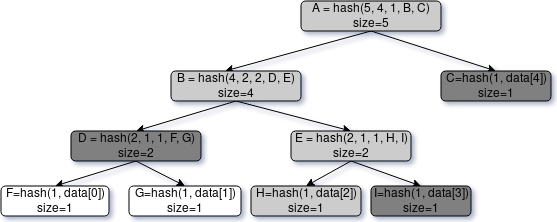
\includegraphics[width=0.7\textwidth]{merkle-tree}
\caption{Example of sized Merkle tree}
\label{fig:merkle-tree}
\end{figure}

To incentivize Witnesses to include private block headers into the public chain,
an Educator should pay some amount of coins per each private block. We should
take into consideration that an educator may be both a local tutor and some big
university. Depending on that, a number of transactions per each block, as well
as paying capacity, may differ. So the cost of a digest publication should
linearly grow with the size of a block. Let the cost for publishing a
public block header be
\begin{equation}\label{sec:priv-chain:pub-cost-eq}
  C_{pub}(B) = \alpha_{pub} + \beta_{pub} \cdot N_{tr}(B)
\end{equation}
, where $N_{tr}(B)$ is the number of transactions in private block $B$ and
$\alpha_{pub}$ and $\beta_{pub}$ are parameters of the network -- a small
constant fee and a linear price coefficient accordingly.

From the description above we can conclude that an educator may have an incentive to lie about the size of the tree. To achieve the ability to prove the number of transactions in the Merkle tree,
we will store the size of the subtree with the hash in each node (as shown in \ref{fig:merkle-tree}). So every transaction disclosure will also verify the size. Suppose that an Educator published a header hash with a wrong size, then every student which is collecting his own fair CV will see that an Educator deceives him, and moreover not a single data-disclosure deal would proceed.

Let's look at the example from the figure \ref{fig:merkle-tree}. Suppose we need to disclose $data[2]$. The path to the node H is $A \rightarrow B \rightarrow E \rightarrow H$. The proof nodes are $C$, $D$, and $I$. So the size of the tree is $$C.size+D.size+I.size+1=5$$


We also consider a possibility for small educators to form pools and release
blocks together in order to reduce costs for each individual educator. See
appendix \ref{apx:pools} for details.
